\section{Monte Carlo Methods}

\subsection{Exercise 5.1}
\subsubsection{Q}
Consider the diagrams on the right in Figure 5.1. Why does the estimated value function jump up for the last two rows in the rear? Why does it drop off for the whole last row on the left? Why are the frontmost values higher in the upper diagrams than in the lower?
\subsubsection{A}
\begin{enumerate}
	\item The value function jumps for the rows in the rear because the player sticks at 20 and 21, where it is unlikely the dealer beat him given her policy to twist for all hands lower than 17.
	\item The value drops when the dealer holds an ace because it can be used to equal either 11 or 1, a stronger position than any of the other hands the dealer could hold.
	\item When an ace is usable, the value function is higher because the player can change the value of his ace from 11 to 1 if she is about to go bust.
\end{enumerate}
$
\hfill \blacksquare
$

\subsection{Exercise 5.2}
\subsubsection{Q}
Suppose every-visit MC was used instead of first-visit MC on the blackjack task. Would you expect the results to be very different? Why or why not?
\subsubsection{A}
The state is blackjack is monotonically increasing and memoryless (sampled with replacement), thus you can never revisit an old state in an episode once it has been first visited. Using every visit MC in this case would have no effect on the value function.
$
\hfill \blacksquare
$

\subsection{Exercise 5.3}
\subsubsection{Q}
What is the backup diagram for Monte Carlo estimation of $q_\pi$?
\subsubsection{A}
\begin{figure}[h!]
	\centering
	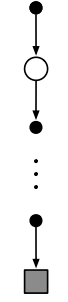
\includegraphics[width=0.05\textwidth]{/chapter5_2}
	\caption{Monte carlo backup diagram for estimation of $q_\pi$ from one episode}
	\label{fig:monte carlo qpi}
\end{figure}
$
\hfill \blacksquare
$

\subsection{Exercise 5.4}
\subsubsection{Q}
The pseudocode for Monte Carlo ES is inefficient because, for each state–action pair, it maintains a list of all returns and repeatedly calculates their mean. It would be more efficient to use techniques similar to those explained in Section 2.4 to maintain just the mean and a count (for each state–action pair) and update them incrementally. Describe how the pseudocode would be altered to achieve this.
\subsubsection{A}
Update formula from section 2.4 is:
\begin{equation}
	Q_n = Q_n + \frac{1}{n}\left[R_n - Q_n\right]
\end{equation}
As we reverse through the episode, we initialise value $N_{s,a}$ for each observed $s$ and $a$ to count the number of visits to the state. Instead of appending $G$ to returns, we use our now initialised $N$, and $G$ to update the value of $Q$. Doing so is more efficient as we don't need to hold a list of all returns which does not scale, we just update using the update rule outlined above.
$
\hfill \blacksquare
$

\subsection{Exercise 5.5}
\subsubsection{Q}
Consider an MDP with a single nonterminal state and a single action that transitions back to the nonterminal state with probability $p$ and transitions to the terminal state with probability $1 - p$. Let the reward be +1 on all transitions, and let $\gamma = 1$. Suppose you observe one episode that lasts 10 steps, with a return of 10. What are the first-visit and every-visit estimators of the value of the nonterminal state?
\subsubsection{A}
For first-visit estimator of the state is the return collected at the end of the episode having visited the first step, assuming we initialise $G=0$:
$
G = 10
$

The every-visit estimator is an average of each of the 10 returns received from the state:
\begin{equation}
G = \frac{1+2+3+4+5+6+7+8+9+10}{10} = 5.5
\end{equation}
$
\hfill \blacksquare
$

\subsection{Exercise 5.6}
\subsubsection{Q}
What is the equation analogous to (5.6) for action values $Q(s,a)$ instead of state values $V(s)$, again given returns generated using $b$?
\subsubsection{A}
Equation 5.6 is as follows:
\begin{equation}
V(s) = \frac{\sum_{t \in \mathcal{T}(s)} \rho_{t:T(t)-1} G_t}{\sum_{t \in \mathcal{T}(s)} \rho_{t:T(t)-1}}
\end{equation}

We only require that $\mathcal{T}$ tracks state action-pairs rather than just states. Equation 5.6 therefore becomes: 

\begin{equation}
Q(s,a) = \frac{\sum_{t \in \mathcal{T}(s,a)} \rho_{t:T(t)-1} G_t}{\sum_{t \in \mathcal{T}(s,a)} \rho_{t:T(t)-1}}
\end{equation}
$
\hfill \blacksquare
$

\subsection{Exercise 5.7}
\subsubsection{Q}
In learning curves such as those shown in Figure 5.3 error generally decreases with training, as indeed happened for the ordinary importance-sampling method. But for the weighted importance-sampling method error first increased and then decreased. Why do you think this happened?
\subsubsection{A}
In the initial episodes, we are unlikely to see episodes from the behaviour policy that match our target policy (i.e. hit for all card sums < 20 and stick thereafter), therefore our estimate for $V(s)$ will remain 0, which happens to be close to our ground truth $V_\pi(s)$. As we see some trajectories from $b$ that match our target policy, variance in our output will be high initially, leading to a higher error, and will drop gradually as we observe further trajectories until it approaches the true value asymptotically after 10,000 episodes.
$
\hfill \blacksquare
$

\subsection{Exercise 5.8}
\subsubsection{Q}
The results with Example 5.5 and shown in Figure 5.4 used a first-visit MC method. Suppose that instead an every-visit MC method was used on the same problem. Would the variance of the estimator still be infinite? Why or why not?
\subsubsection{A}
The variance of the estimator would remain infinite, as the expected return is still 1 for every-visit to the state. The only difference between first-visit and every-visit MC in this case is that the number of terms increases $\alpha$ to the number of visits to the state and so would continue to run to infinity.
$
\hfill \blacksquare
$

\subsection{Exercise 5.9}
\subsubsection{Q}
Modify the algorithm for first-visit MC policy evaluation (Section 5.1) to use the incremental implementation for sample averages described in Section 2.4. 
\subsubsection{A}
\begin{figure}[h!]
	\centering
	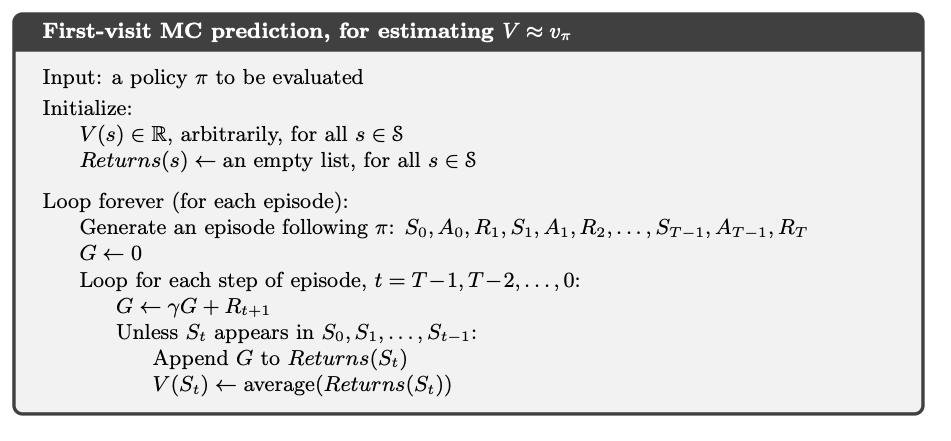
\includegraphics[width=0.75\textwidth]{/ex5.9}
	\label{fig:monte carlo policy eval}
\end{figure}

Modifying the above to include sample averages we change the last two lines. Instead of appending $G$ to $Returns(S_t)$ and averaging, we update $V(S_t)$ directly using:
$
V(S_t) = V(S_t) + \frac{1}{n}\left[G - V(S_t)\right]
$

to do this we need to initialise a new variable $n$ that counts the number of cross-episode visits to state $S_t$.
$
\hfill \blacksquare
$

\subsection{Exercise 5.10}
\subsubsection{Q}
Derive the weighted-average update rule (5.8) from (5.7). Follow the pattern of the derivation of the unweighted rule (2.3).
\subsubsection{A}
We have $C_o = 0$ and $C_n = \sum_{k=1}^{n} W_k$. Therefore:
\begin{align}
V_{n+1} &= \frac{\sum_{k=1}^{n}W_k G_k}{C_n}\\
V_{n+1}{C_n} &= \sum_{k=1}^{n}W_k G_k \\
V_{n+1}{C_n} &= W_n G_n + \sum_{k=1}^{n-1}W_k G_k \\
V_{n+1}{C_n} &= W_n G_n + V_n \sum_{k=1}^{n-1}W_k \\
V_{n+1}{C_n} &= W_n G_n + V_n C_{n-1} \\
V_{n+1}{C_n} &= W_n G_n + V_n \left(C_n - W_n\right) \\
\vdots \\
V_{n+1} &= V_n + \frac{W_n}{C_n}\left[G_n - V_n\right] \\
\end{align}
$
\hfill \blacksquare
$

\subsection{Exercise 5.11}
\subsubsection{Q}
In the boxed algorithm for off-policy MC control, you may have been expecting the $W$ update to have involved the importance-sampling ratio $\frac{\pi (At|St)}{b(At|St)}$, but
instead it involves $\frac{1}{b(At|St)}$. Why is this nevertheless correct?
\subsubsection{A}
Because our policy $\pi(S_t)$ is a deterministic, greedy one, we are only observing trajectories where $\pi(A_t | S_t) = 1$, hence the numerator in the equation = 1.
$
\hfill \blacksquare
$

\subsection{Exercise 5.12}
\ProgrammingExercise
$
\hfill \blacksquare
$

\subsection{Exercise 5.13}
\subsubsection{Q}
Show the steps to derive (5.14) from (5.12). 
\subsubsection{A}
5.12 is:

\begin{align}
\rho_{t:T(t)-1} R_{t+1} &= R_{t+1} \prod_{k = t}^{T-1} \frac{\pi(A_k | S_k)}{b(A_k | S_k)} \\
\end{align}
$
\hfill \blacksquare
$

\subsection{Exercise 5.14}
\subsubsection{Q}
Modify the algorithm for off-policy Monte Carlo control (page 111) to use the idea of the truncated weighted-average estimator (5.10). Note that you will first need to convert this equation to action values.
\subsubsection{A}
...
$
\hfill \blacksquare
$
